% Made up for the tikra benchmark.
\usetikzlibrary{decorations.pathmorphing, decorations.markings}
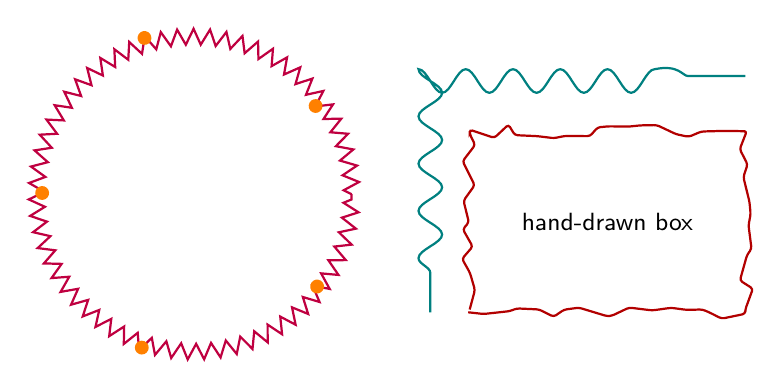
\begin{tikzpicture}[thick]
  \draw[purple, decorate, decoration={zigzag, segment length=2mm, amplitude=1mm},
      postaction={decorate, decoration={markings, mark=between positions 0.1 and 0.9 step 0.2 with {\fill[orange] circle (2.5pt);}}}]
    (0,0) circle (2);
  \draw[teal, decorate, decoration={snake, amplitude=1.5mm, segment length=6mm, pre length=5mm, post length=5mm}]
    (3,-1.5) -- (3,1.5) -- (7,1.5);
  \draw[red!70!black, decorate, decoration={random steps, segment length=2mm, amplitude=1mm}, rounded corners=1pt]
    (3.5,-1.5) rectangle (7,0.8);
  \node[font=\sffamily\small] at (5.25,-0.35) {hand-drawn box};
\end{tikzpicture}
